\section{Problem Definition} \label{sec:prob}
In this section, we describe the necessary background knowledge and highlight the identified two performance issues: 1) long execution paths of the guest page table (de)allocation and 2) the additional IOTLB flushes.
As Xen~\cite{XEN-SOSP03} is a typical and popular paravirtual hypervisor, we use Xen in a x86 MMU model~\cite{x86-pv-model} to illustrate the details.
The presented or similar mechanisms are available on the other paravirtual settings.


\subsection{Long Execution Path}\label{sec:longpath}
The long execution path issue refers to the execution paths for the guest page table page allocation and deallocation.
In the existing design, allocating and deallocating a page table page are time costly, as they have to invoke the complex memory allocators and performance both software (i.e., page table) and DMA validations.
%In addition, the DMA validations always lead to additional IOTLB flushes, which would reduce the DMA address translation speed and may consequently lower the I/O performances.
In addition, such allocation and deallocation events frequently occur in the system, i.e., the numerous process creations and exits will result in many page-table page allocations and deallocations.
Thus, it is necessary to deeply understand the long execution path issue and improve the performance accordingly.

\subsubsection{Page Allocation and Deallocation}
To allocate a page, the guest kernel has to invoke the system allocators, typically from slab allocator to buddy allocator.
The slab allocator~\cite{slaballocator} consists of a variable number of caches that are linked together on a doubly linked circular list.
Each cache maintains blocks of contiguous pages in memory called slabs, which are carved up into small chunks for the data structures and objects.
When \emph{kmalloc} is called, all it does is searching through the prepared caches.
If there is no suitable object, the buddy allocator will be involved.
The Buddy allocator~\cite{buddyallocator} manages all free pages that are allocated in blocks with the sizes of powers of 2.
When the allocation function is invoked, it first searches for blocks of pages of the size requested following the chain.
If no blocks of the requested size are free, blocks of the next size (which is twice that of the size requested) are looked for.
This process continues until all of the free area has been searched or until a block of pages has been found.

In contrast to the page allocation, the page deallocation is to return the page back to the system.
The deallocation process may also invoke slab allocator and/or buddy allocator, and would trigger the updates of the corresponding data structures,
e.g., the buddy allocator always attempts to recombine the freed pages into larger blocks.

In brief, the page allocation and deallocation are time costly due to the deep invocations and complex updates of the dependent data structures.


\subsubsection{Page Table Validations}\label{sec:pv-security}
Page tables are used by a hardware, i.e., Memory Management Unit (MMU), to translate the linear addresses into physical addresses used by the hardware to execute instructions.
In the PAE-enabled paging mode, a page table has three levels: L1 level (bottom level), L2 level (middle level) and L3 level (top level).
The slots in L1, L2 and L3 levels are known as Page Table Entry (PTE), Page Middle Directory (PMD) and Page Global Directory (PGD), respectively.
A PTE slot could determine the access permissions of a page, e.g., the kernel could set a page as read-only by clearing the bit within a PTE slot that represents the writable permission.
Typically, each user process has its own page table, and the creation and exit of a user process will be accompanied by the allocation and deallocation of a page table respectively.
\begin{figure}[ht]
\centering
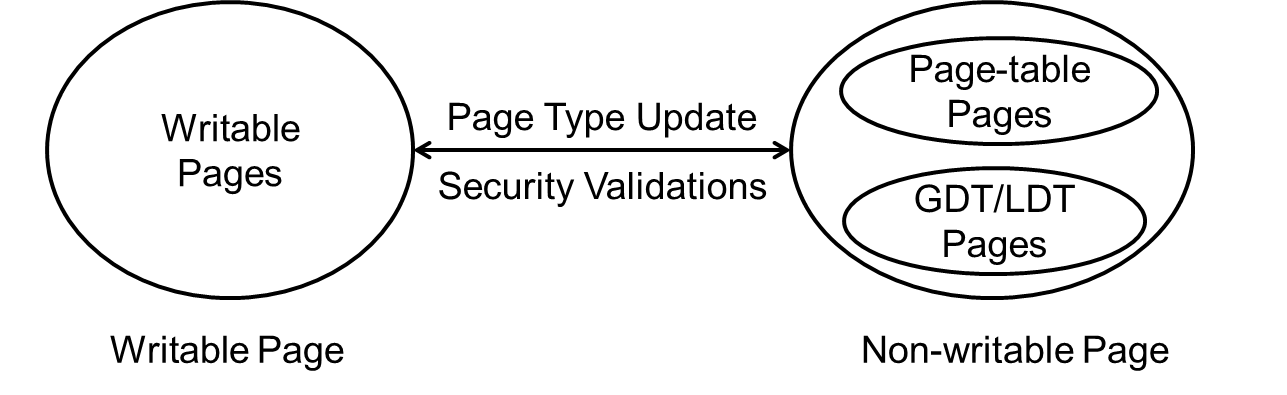
\includegraphics[width=0.45\textwidth]{image/background/page-type-update.png} \\
\caption{Page type updates between writable pages and non-writable pages. }
\label{fig:page-type-updates}
\end{figure}


%In order to ensure that the guest cannot subvert the system, the hypervisor requires that certain update policies are maintained,
%and thus all updates of the page tables should be vetted by the hypervisor.
%To this end, the guest OS is deprivileged, from ring-0 to ring-1, leaving ring-0 for the Xen hypervisor.
%This prevents the guest OS from executing privileged instructions, e.g., the guest OS cannot directly update control registers.

The hypervisor defines two page types 1) \emph{writable page} that is writable for software and DMA, and 2) \emph{non-writable page} that is non-writable for both software and DMA.
The non-writable page has several sub-page types, such as page-table page and GDT/LDT pages.
In addition, the hypervisor also requires that every page type update only occur between writable and non-writable pages, as summarized in Figure~\ref{fig:page-type-updates}.
The hypervisor maintains a type reference count for each page, and enforces the policy that any given page has exactly one type at any given time.
In addition, it also enforces that only pages with the writable type have a writable mapping in the page tables.
By doing this it can ensure that the guest OS is not able to directly modify any page-table pages and therefore cannot subvert the security of the whole system.

Whenever a page table is loaded to work, there should be a page type update from writable page to non-writable page (i.e., page-table page).
First, the hypervisor must ensure the L3 page-table page has a type count of zero.
In addition, it must be validated to ensure that it follows the following policy:
for a page with a page-table type to be valid, it is required that any pages referenced
by a present page table entry in the page have the type of the next level down.
For instance, any page referenced by a page with type L3 Page Table must itself have the type L2 Page Table.
This policy is applied recursively down to the L1 page table layer.
At L1 the invariant is that any data page mapped by a writable page table entry must have the writable page type.
By applying these policies, Xen ensures that all page-table pages as a whole are safe to be loaded.
The hypervisor also verifies all slots of the page table to ensure that the mappings and access permissions are correct and expected.
Note that the hypervisor is always involved in all updates of the page tables, the policies on the page table updates are non-bypassable.

The validation process in the page table deallocation is contrary to the one in the page table allocation.
In brief, the hypervisor will validate the page table's type count, access permissions and the slot mappings to ensure that the page table is completely and securely deallocated.

\subsection{DMA Validations and IOTLB Flushes}
\subsubsection{DMA Address Translation}
The input/output memory management unit (IOMMU)~\cite{intelvt} is a memory management unit (MMU) that connects a DMA-capable I/O bus to the main memory.
Like a traditional MMU, the IOMMU maps device addresses (also called as I/O addresses) to physical addresses through a dedicated page table.
%This technique is also known as DMA remapping.
The IOMMU page table that is created and maintained by the hypervisor in its own space is able to restrict the access on a particular page by configuring the permission bits.
The hypervisor grants different access permissions for different page types, such as the writable pages are always allowed with full access permissions, while the page-table pages are always inaccessible to any devices.

However, if the DMA address translation always needs to look up the IOMMU page table, it will be slow and inefficient.
To accelerate the translation speed, the I/O translation look-aside buffer (IOTLB) is introduced.
The IOTLB is used to cache frequently accessed page table entries.
By doing so, the IOTLB is very likely to be accessed, indicating that the physical address of a queried DMA address will be immediately fetched through the IOTLB path (Figure~\ref{fig:iotlbpath}).
If unlikely the IOTLB miss occurs, the DMA address translation still can go the slow I/O page-table path to get the physical address (Figure~\ref{fig:ioptpath}).
To achieve a better I/O performance, the DMA address translation should avoid taking the I/O page-table path as far as possible.

\begin{figure}[!t]
    \begin{subfigure}{0.45\textwidth}
        
\includegraphics[width=1\textwidth]{image/background/DMA-IOTLB-translation.png}
        \caption{\centering IOTLB Path.}
        \label{fig:iotlbpath}
    \end{subfigure}
    \vfill
    \begin{subfigure}{0.45\textwidth}
        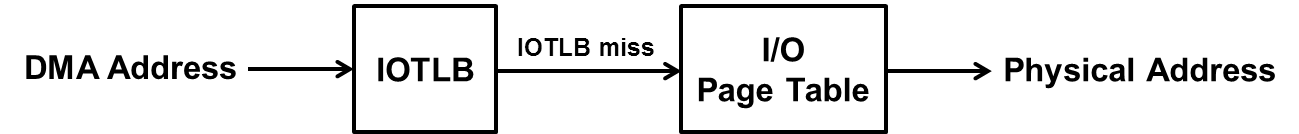
\includegraphics[width=1\textwidth]{image/background/DMA-pt-translation.png}
        \caption{\centering I/O Page-Table Path.}
        \label{fig:ioptpath}
    \end{subfigure}
    \caption{IOTLB path is much faster than I/O page-table path.}
    \label{fig:dma-add-trans}
\end{figure}


\subsubsection{Additional IOTLB Flushes}
%In paravirtualization, the writable page is writable for DMA requests, while the non-writable page (e.g., the page table page) is non-writable for DMA requests.
The page table allocation and deallocation always trigger the updates between the writable pages and the page-table pages, and they have different access permission for DMA requests.
To keep the security of the hypervisor, the DMA validation is necessary.
Specifically, the hypervisor will update the corresponding entries of the IOMMU page table to set correct access permissions.
After this, the hypervisor also needs to flush IOTLB entries to invalidate the old entries, without which the security of the hypervisor would be violated, e.g., the DMA requests could write the page-table pages through stale IOTLB entries.

\begin{figure}[ht]
\centering
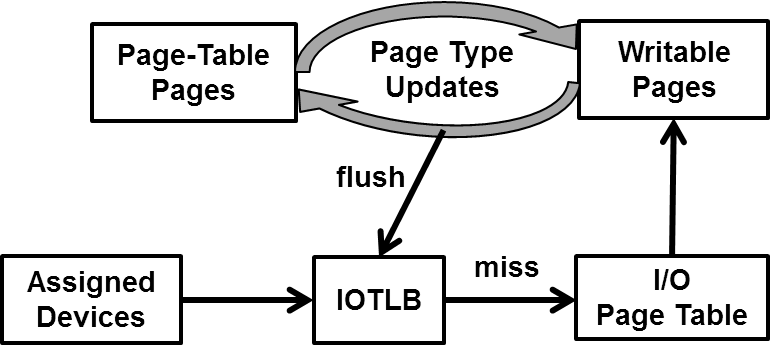
\includegraphics[width=0.45\textwidth]{image/background/problem-illustration.png} \\
\caption{The DMA validations in page type updates introduce additional IOTLB flushes, which lead to selecting the slow path  (i.e., I/O page-table path) of the DMA address translation.}
\label{fig:pro-ill}
\end{figure}


In addition, the additional IOTLB flushes are likely to let the DMA address
translations take the slow and inefficient page-table path,
instead of taking the fast and efficient IOTLB path (Figure~\ref{fig:pro-ill}), due to the additional IOTLB misses.
Numerous IOTLB misses would lower the speed of the DMA transferring, especially for the high performance devices, such as the Intel I/OAT ~\cite{lauritzenintel}.
%Moreover, the DMA validations are frequently triggered if there are many creations and exits of user processes due to certain cases.
%In fact, it


%In brief, we summarize all these into three key points, which are listed as follows:
%\begin{enumerate}
%\item (O1) Each page-type change triggers the invalidation of at least one IOTLB entry.
%\item (O2) The main source of causing IOTLB flush is the page-type changes between writable pages and page-table pages (see figure~\ref{fig:pro-ill}).
%\item (O3) The additional IOTLB flushes inevitably have negative impacts on the I/O performance of the peripheral devices.
%\end{enumerate}


